\sect{5. How to play}

You are a kung-fu fighter fighting through five stages, from the temple hall to a mountain pass. Each stage has
several floors: go up with \key{$\uparrow$}, drop down with \key{$\downarrow$}. On every stage the same plan applies:

\begin{enumerate}
\item \textbf{Beat the 21 enemies} that come out of the two doors and from the sides. Kick them down; a jump kick scores more.
\item When the last of the wave is down, the \textbf{boss} of the stage appears. Hit it \textbf{five times} to beat it.
\item Beat the boss and the stage is clear: your \textbf{GUTS!} bonus is counted and the next \texttt{STEP} begins.
\end{enumerate}

After the fifth stage the game starts again from the first, with faster and more aggressive enemies. From the second round on, a \textbf{bird} flies over the stage now and then and \textbf{drops a rock}: step aside.

Some enemies carry a \textbf{power-up ball}. Knock down the carrier to get a special weapon for a while.

Each stage has a time limit. When little time is left a \texttt{HURRY UP} banner appears, and when it runs out you lose a life (\texttt{TIME OVER}). The more enemies there are to beat, the more time you are given.

% ==================================================================
\sect{6. The status panel (HUD)}

\begin{figure}[H]
\centering
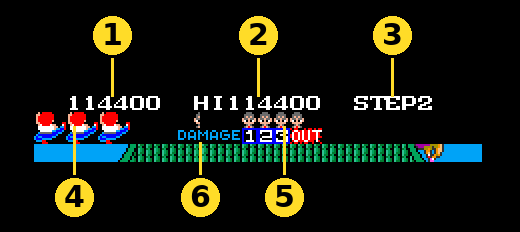
\includegraphics[width=\textwidth]{img/hud.png}
\caption{The status panel at the top of the screen.}
\end{figure}

\begin{tabularx}{\textwidth}{@{}cp{3.1cm}X@{}}
\toprule
\textbf{\tNo} & \textbf{\tElement} & \textbf{\tTellsYou}\\
\midrule
1 & Score & Your score.\\
2 & High score & The best score of the high-score table.\\
3 & Stage & \texttt{STEP} and the number of the stage, counting the rounds (after the fifth stage comes \texttt{STEP 6}).\\
4 & Lives & One icon for each spare life; with five or more it shows one icon and the number.\\
5 & Enemies left & Each small head stands for three enemies still to beat in the wave; it shortens as you win.\\
6 & Damage & \texttt{DAMAGE 1 2 3 OUT}: each hit lights one more number, and the current one blinks. The fourth hit, \texttt{OUT}, costs a life.\\
\bottomrule
\end{tabularx}

% ==================================================================
\sect{7. Scoring and lives}

\begin{center}
\begin{tabular}{@{}lr@{}}
\toprule
\textbf{Action} & \textbf{Points}\\
\midrule
Kick an enemy & 200\\
Jump kick & 500\\
Combo (second knock-out in quick succession) & 1000\\
Make the bonus object appear & 500\\
GUTS! bonus, for each unused damage level & 1000\\
\bottomrule
\end{tabular}
\end{center}

\begin{itemize}
\item You start with \textbf{3 lives}.
\item You earn an \textbf{extra life at 40\,000 points and then every 80\,000}.
\item The difficulty is the one you choose at the title screen, \textbf{hard} (\key{1}) or \textbf{medium} (\key{2}), and grows with every stage you clear.
\item After \texttt{GAME OVER}, the eight best scores are kept in the \textbf{high-score table}, with your three initials: change the letter with left and right, and kick to accept it. The table starts with the names \texttt{MSX}, \texttt{BTV}, \texttt{DI}, \texttt{HLT}, \texttt{KON} and \texttt{AMI}.
\end{itemize}

\begin{figure}[H]
\centering
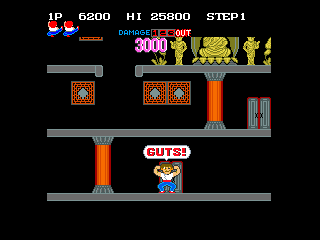
\includegraphics[width=0.48\textwidth]{../img/guts.png}\hfill
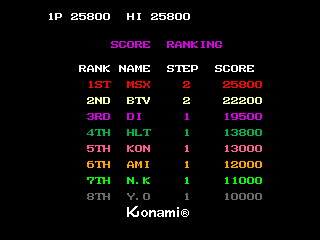
\includegraphics[width=0.48\textwidth]{../img/ranking.png}
\caption{Left: the \texttt{GUTS!} bonus at the end of a stage. Right: the high-score table.}
\end{figure}

% ==================================================================
\sect{8. Tips}

\begin{itemize}
\item Keep moving: enemies surround you. Fight with your back to a wall or a door only when you have room to retreat.
\item A kick has a short reach. Let the enemy come close and kick as it arrives.
\item The jump kick scores 500 against 200 for a kick and crosses gaps, but leaves you exposed while you are in the air.
\item Use up and down to change floor, and look at which enemies wait on the floor you are heading for.
\item Keep your damage low: every level you do not use is worth \textbf{1000 points} when the stage is clear.
\item Watch the head icons: when only a few are left, the boss is close.
\item From the second round on, look up when you hear the bird.
\item Always read the time: with \texttt{HURRY UP} on screen, go straight for the remaining enemies.
\end{itemize}
